\documentclass[a4paper,11pt]{article}
\usepackage[T1]{fontenc}
\usepackage[utf8]{inputenc}
\usepackage{lmodern}
\usepackage[francais]{babel}
\usepackage[ portrait, margin = 0.7 in]{geometry}
\usepackage{amsmath}
\usepackage{graphicx}
\graphicspath{{./images/}}
\usepackage{float}
\usepackage{subfig}
\usepackage{mathrsfs}
\usepackage{gensymb}
\numberwithin{equation}{section}


\begin{document}

\title{\LARGE \bf Mesure de la rotation différentielle du Soleil}
\author{MERCIER Wilfried - Observatoire de Paris}
\maketitle


\section{Introduction}
\subsection{Rotation différentielle du Soleil}
Un corps non solide comme une étoile ou une atmosphère planétaire possède une vitesse de rotation qui peut varier avec la latitude. On dit que le corps possède une rotation différentielle. Dans notre cas, on s'intéresse au Soleil et on souhaite déterminer sa vitesse de rotation pour plusieurs latitude à l'aide d'images de celui-ci.\newline Pour ce faire il faut déterminer la position d'un point à la surface du Soleil et suivre son déplacement au fil du temps.
\subsection{Utilité des tâches solaires}
Afin de pouvoir mesurer la vitesse d'un point à la surface du Soleil il faut que celui-ci ait un contraste élevé avec la photosphère. On choisit de regarder les tâches solaires qui sont des zones plus froides et donc plus sombres par rapport à la photosphère résultant de la déformation de boucles de champs magnétiques. Celles-ci restent en réalité fixes par rapport à la photosphère. Ainsi en étudiant leur mouvement on étudie en réalité le mouvement de rotation du Soleil à différentes lattitudes.


\section{Étapes clés du projet}
\subsection{Sélection des images}
Afin d'étudier la rotation différentielle du Soleil il faut pouvoir trouver un certain nombres d'images tel que l'on ait les conditions suivantes respectées:
\begin{itemize}
  \item avoir des tâches solaires bien visibles qui traversent l'image
  \item avoir plusieurs tâches solaires à différentes latitudes à étudier
\end{itemize}
La première condition est respectée si on considère la bande CaII Klv. On choisit donc des images du spectrohéliographe de Meudon dans cette bande-ci sur le site BASS2000.

\subsection{Réglage du contraste}
Pour détecter facilement les tâches et les bords du Soleil on souhaite maximiser le contraste. Pour ce faire on produit un histogramme des couleurs de l'image et on cherche la zone dans laquelle les couleurs sont le plus regroupées (hors fond noir).\newline
On cherche la valeur maximale $im_{max}$ de l'image puis on découpe l'ensemble des couleurs en 100 intervalles entre 0 et $im_{max}$. En parcourant l'image on rempli alors l'histogramme.\newline
Dans le cas de l'image de référence on remarque que l'histogramme est constitué de deux zones: une en dessous de $1000$ due au fond noir et une seconde autour de $8000$ correspondant à la photosphère. \newline
Augmenter le contraste revient à trouver les valeurs des couleurs minimale ($c_{min}$) et maximale ($c_{max}$) à l'affichage. Celles-ci vont se trouver de part et d'autre du second pic. Pour les déterminer on cherche la couleur avec la fréquence d'apparition maximale $f_{max}$ dans l'histogramme et on regarde les deux valeurs avec une fréquence $f_{max}/n$, où n est un paramètre à ajuster.\newline
On prendra $n \approx 20$ dans la suite du programme.

\begin{figure}[H]
  \centering
  \subfloat[Histogramme complet de l'image de référence.\newline On voit deux zones distinctes apparaître: une en-dessous \newline de $1000$ et une
            autour de $8000$.]{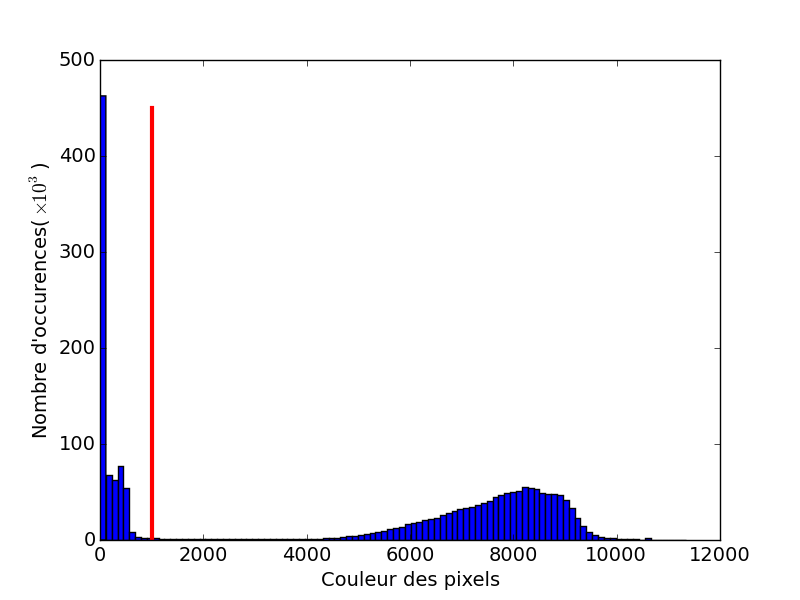
\includegraphics[width=0.48\linewidth]{histogramme}}
  \subfloat[Histogramme recentré autour de 8000. On voit deux valeurs pour lesquelles la fréquence d'apparition
            dans l'image est une fraction $n$ de la fréquence maximale.]{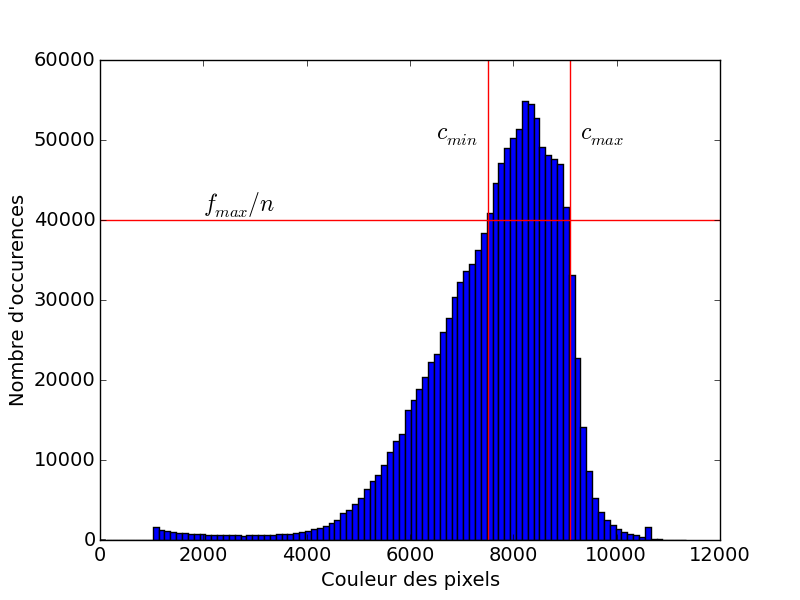
\includegraphics[width=0.48\linewidth]{histogramme_corr}}
  
   \caption{Histogrammes de l'image de référence avant et après analyse des couleurs minimales et maximales pour l'affichage}
\end{figure}


\subsection{Remise à l'échelle et recentrage}
Pour des questions de praticabilité on décide d'appliquer un facteur d'échelle à l'image. On défini une nouvelle image dont les dimensions sont divisées d'un facteur d'échelle $ech$. À chaque nouveau pixel correspond une nouvelle valeur moyennée sur un carré de dimensions $ech\times ech$ pixels

\begin{equation}
  \text{nouvelle valeur} = \frac{1}{ech^2} \sum_{i=1}^{ech} \sum_{j=1}^{ech} (\text{ancienne valeur})_{ij}
\end{equation}

On répète l'opération en se décalant de $ech$ pixels et ainsi de suite de gauche à droite et bas en haut. Éventuellement si la taille orginelle de l'image n'est pas un multiple du facteur d'échelle on supprime les bords.\newline
Pour pouvoir déterminer le rayon du Soleil en pixels on souhaite recadrer l'image. On cherche donc les bords du Soleil en parcourant l'image dans 4 zones restreintes (deux centrées verticalement et deux horizontalement). Dans ces zones les premiers pixels rencontrés seront noirs et le premier pixel "blanc" découvert correspondra à un des bords du Soleil. Cependant pour éviter de détecter n'importe quel pixel non-noir on cherche plutôt le premier pixel dans la zone ayant une couleur d'au-moins 30\% du maximum de l'image.

\subsection{Passage aux coordonnées sphériques}
L'image obtenue nous fournit les coordonnées de la tâche dans le plan de l'image. Or on souhaite déterminer la vitesse de rotation de la tâche, ce qui nécessite de passer dans un système de coordonnées physiques: les coordonnées sphériques.\newline
On considère que l'image du Soleil se trouve dans le plan $(yOz)$. Ainsi d'après les formules usuelles des coordonnées sphériques on a les relations:

\begin{equation}
  y = R_{\odot} \cos l \sin \mathscr{L} \qquad  z = R_{\odot} \sin l
\end{equation}

où $R_{\odot}$ est le rayon du Soleil en pixels, $l$ la latitude de la tâche, $\mathscr{L}$ la longitude de la tâche et où les coordonnées $(y,z)$ sont les coordonnées de la tâche sur l'image en pixels dans le repère centré sur le Soleil (y horizontale, z verticale).\newline
Ainsi en inversant ces deux relations on obtient

\begin{equation}
  \label{eq:coord}
  l = \arcsin \frac{z}{R_{\odot}} \qquad \mathscr{L} = \arcsin \frac{y}{R_{\odot} cos l}
\end{equation}

\begin{figure}[H]
  \centering
  \subfloat[Graphe de la longitude d'une tâche à une lattitude\newline de 15\degree en fonction du temps. Les points représentent les\newline données et le trait 
            continu le fit obtenu par régression\newline linéaire]{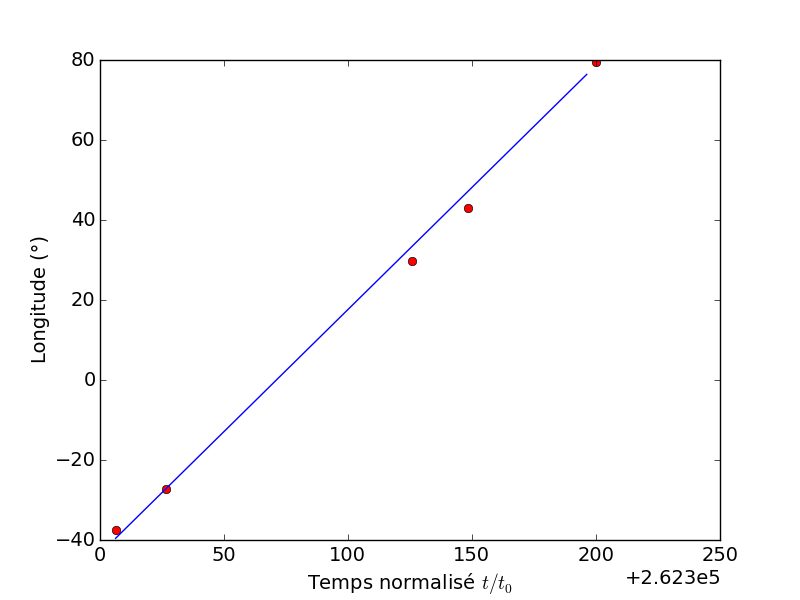
\includegraphics[width=0.48\linewidth]{rotation}}
  \subfloat[Rotation différentielle du Soleil en fonction de la latitude. On observe une valeur plus élevée de rotation vers l'équateur.]{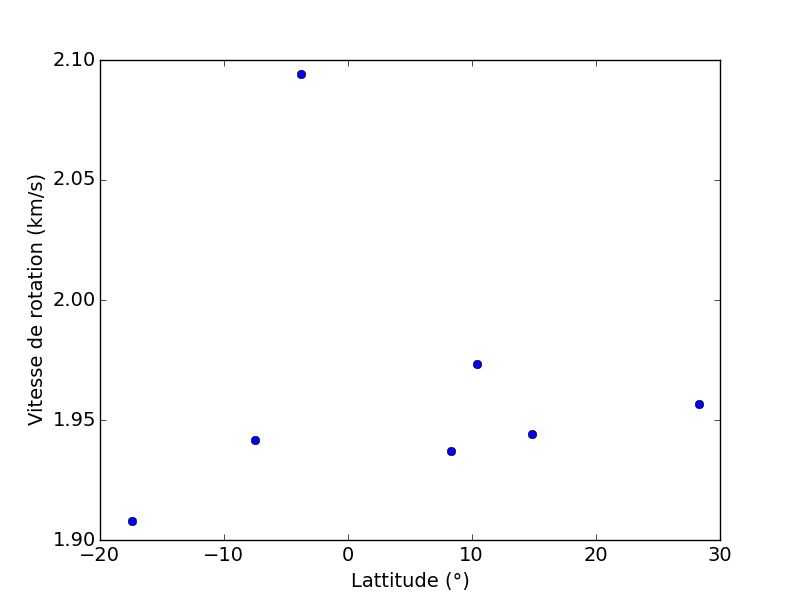
\includegraphics[width=0.48\linewidth]{vit_rot}}
 
  \caption{Résultats obtenus pour la mesure de la rotation différentielle du Soleil.}
  \label{fig:graphe}
\end{figure}

\section{Résultats}
\subsection{Régression linéaire et rotation différentielle}
Les coordonnées ont été mesurées pour 7 tâches sur 5 jeux d'images. Pour chaque tâche les coordonnées sphériques et le temps sont stockées et une régression linéaire est effectuée avec \textit{reglin\_Mercier}. Les régression linéaires sont toutes très correctes et fournissent des coefficients de corrélation de l'ordre de $0.99$.
La pente de la régression correspond à la vitesse de rotation $\omega$ (rad/s). On obtient la période de rotation via 

\begin{equation}
  \label{eq:periode}
  T(j)= \frac{2\pi}{3600 \times 24 \times \omega}  
\end{equation}

Et on a la vitesse de rotation en km/s en multipliant la vitesse de rotation par un rayon modulé $R_{\odot} \cos(l)$ puisque la tâche se déplace à lattitude constante. Pour une tâche quasiment sur l'équateur on obtient une période de rotation de $24\text{j}3\text{h}$ et pour une tâche à environs $30$\degree de lattitude on obtient $22\text{j}9\text{h}$. Comme on peut le voir sur la figure \ref{fig:graphe}b la vitesse de rotation est plus élevée à l'équateur et semble diminuer en s'éloignant. Les résultats en terme de période de rotation et de vitesse de rotation sont consistants avec les valeurs réelles compte tenu des incertitudes sur la vitesse qui doivent être assez grandes.

\subsection{Incertitudes sur la période}
Compte tenu de Eq.\ref{eq:periode} on s'attend à avoir une erreur sur la période de rotation $\Delta T / T =   \Delta \omega / \omega$. Pour la rotation à l'équateur après avoir moyenné l'ensemble des erreurs on trouve $\Delta T \approx 9 \text{h}$.\newline
On peut aussi étudier comment l'erreur sur le rayon et les coordonnées sphériques se répercute dans la période. Pour le rayon du Soleil on observe qu'en partant d'un seuil de 0.3 le rayon du Soleil change notablement (plus d'un pixel) à partir de 0.6 d'environ $10$px. On prendra donc $\Delta R_{\odot} = 10\text{px}$ par la suite. De plus du fait que les tâches sont étalées, des erreurs sur les coordonnées $(y,z)$ vont apparaître quand on clique de l'ordre de $10$px aussi.\newline
D'après Eq.\ref{eq:coord} on a alors les erreurs suivantes sur les coordonnées sphériques

\begin{equation}
  \Delta l = \frac{\sin l}{\cos l} \left [\frac{\Delta z}{z} + \frac{\Delta R}{R} \right ] \qquad \Delta L = \frac{\sin L}{\cos L} \left [\frac{\Delta y}{y} + \frac{\Delta R}{R} + \frac{\sin l}{\cos l}\Delta l \right ]
\end{equation}

On peut borner les erreurs. Par exemple le point le plus haut est à $30$\degree, ce qui donne $\Delta l < 2.5 \degree$ et $\Delta L < 15 \degree$. Cependant de telles erreurs dépendent de la position de la tâche et seront plus accentuées vers les pôles. La valeur obtenue pour l'équateur semble donc la plus juste de toutes.


\newpage
\appendix
\section{Annexe : notice d'utilisation des programmes}
\subsection{Programme principal \textit{Mercier\_programme.c}}
Partie principale du programme qui appelle \textit{affiche.c}, récupère les coordonnées sphériques et le temps retournés par ce dernier et les stocke dans des tableaux. Une régression linéaire est effectuée par \textit{reglin\_Mercier} et les paramètres de la régression ainsi que le coefficient de corrélation et l'erreur sont affichés.\newline
Les images à traiter sont fournies en argument dans un fichier.

\subsection{Module \textit{affiche.c}}
Partie secondaire du programme qui contient le cube de données et appelle successivement les routines de traitement d'image et de calcul de coordonnées puis retourne les coordonnées sphériques et le temps. Dans l'ordre on trouve \textit{histogramme.c}, \textit{reduction.c}, \textit{recadrage.c}, \textit{coord\_sph.c}.

\subsection{Module \textit{histogramme.c}}
Sous-programme qui détermine un histogramme de l'image et supprime les valeurs dans l'histogramme dont la couleur est en-dessous de 1000. La fonction \textit{correction\_histogramme} se charge de déterminer les deux couleurs $c_{min}$ et $c_{max}$ telles qu'elles aient une valeur $n$ fois inférieure à celle ayant la fréquence d'apparition maximale (couleur du maximum de l'histogramme), avec $n$ un paramètre ajustable.\newline
Ce programme retourne $c_{min}$ et $c_{max}$.

\subsection{Module \textit{reduction.c}}
Ce sous-programme se charge de réduire d'un facteur d'échelle $ech$ les dimensions du cube originel afin qu'il puisse s'afficher en entier à l'écran. Il retourne un nouveau cube avec les dimensions réduites.

\subsection{Module \textit{recadrage.c}}
Module qui détermine les 4 bords du Soleil en évitant au maximum de rencontrer soit les écritures dans le bord haut gauche de l'image, soit les 4 indicateurs N, S, W, E sur certaines images. Il se charge de remplir un nouveau cube où seulement les pixels dans la région délimitée par les 4 bords sont gardés.\newline
Il retourne le nouveau cube une fois complété.

\subsection{Module \textit{coord\_sph.c}}
Dernier sous-programme appelé par \textit{affiche.c}. Il se charge d'une part de calculer les nouvelles coordonnées de la tâche cliquée dans le repère centré sur le Soleil, et d'autre part de transformer ces coordonnées en coordonnées sphériques $(l, \mathscr{L})$.\newline
Il retourne les nouvelles coordonnées sphériques.

\subsection{Header \textit{affiche.h}}
Contient la déclaration de la fonction principale du fichier \textit{affiche.c} appelée par \textit{Mercier\_programme.c}.

\subsection{Header \textit{fonctions.h}}
Contient les déclarations des fonctions appelées par le module \textit{affiche.c} (traitement d'images et coordonnées).



\end{document}
